\documentclass[11pt]{article}
\usepackage[utf8]{inputenc}
\usepackage[english]{babel}
\usepackage[T1]{fontenc}
\usepackage{gb4e+}
\usepackage{graphicx}


\title{Automatic register annotation?}

\begin{document}
\maketitle

\section{Introduction}

Motivation: Variation, Biber, Bigbert \& automatic register classification based on docuement-level counts of linguistic features; efforts to automatically generate document-level genre/register meta data based on such data.
Aim: demonstrate more appropriate use of linguistic features in variational linguistic research;
Outline: Present Biber-like feature extraction software for German; extract document-level features from corpora of newspaper and web texts; aggregate features via factor analysis; 
In 3 short case studies of (possibly register sensitive) morpho-syntactic variation phenomena, compare the „explanatory“ power of the resulting factors to that of (selected) raw features, i.e., not using aggregation. 

Clarification \#1: we do not advocate ``fishing'', ``snooping'', ``hunting'': in practice, if the  study is not explicitly declared as explorative, researchers should approach a given phenomenon with clear idea of which variables are relevant, based on ``substantive theory''.

Clarification \#2: The case studies presented here are merely intended to highlight the differences between models using aggregated data and models using non-aggregated data. So we focus on the automatically extracted linguistic features, deliberately neglecting other factors that can be expected to play a role in modeling a given phenomenon.


\section{The COReX feature extractor}

COReX is a piece of software that extracts a large number of normalised linguistic feature counts at the document level from German text.1 It does not perform any linguistic annotation by itself, but instead requires linguistic pre-processing, typically performed automatically by dedicated annotation tools. The input format is vertical text (one token per line) with token level annotations in columns 2 through n, and token spans represented as XML-elements (this corresponds to the input format required by tools such as OpenCWB and NoSketchEngine). Required XML-elements are doc (document) and s (sentence). In order to extract the full range of features, the data must include part-of-speech tags (STTS, REF), morphological features (MarMoT, REF),named entity annotations (Stanford NER, REF) as well as topological field annotations (Berkeley, REF). For some annotation layers, such as morphological features and topological fields, a particular formatting is required. COReX outputs a modified version of the input data where normalised document-level feature counts are added as attribute-value pairs to the opening <doc > tag for each document. Moreover, a number of non-normalised counts (such as perfect and passive) are added as attribute-value pairs to the <s > tag for each sentence. Features include non-linguistic categories such as mean word length and mean sentence length; counts for individual parts-of-speech; ...
 
[Distribution of features in COW data; clustering]

\section{Aggregation: factor analysis}

Brief summary, this is meant to be illustrative for a number approaches to aggregation; chosen because it has played a prominent role in (one strand of) variation / register research

\section{Case studies}
In this section, we explore the consequences of aggregating individual linguistic predictors into more abstract factors, for the purpose of modeling linguistic alternation phenomena. In a series of case studies, we model particular morpho-syntactic alternation phenomena with generalized linear models (GLMs), using only document-level information. Each time, we use as predictors the full set of linguistic feature counts as extracted by COReX. In addition, we specify an alternative model using as predictors the per-document factor loadings from a factor analysis. Finally, we compare these models wrt. to model fit and prediction accuracy. 
We are aware that some or all of the phenomena could probably be better explained / modelled if other kinds of predictors were taken into account as well (e.g., lexical information, syntactic properties at various levels). However, since we are interested in what different sorts of document-level information can contribute to modelling the alternation phenomena, we deliberately ignore other predictors as part of our study design.


\subsection{Dative vs genitive case governed by prepositions}

A number of prepositions in German show variation wrt. case marking of their NP complement. A well-known example is the accusative/dative alternation after certain prepositions, which systematically encodes a semantic distinction (directional/non-directional; REF). In the present case study, we will be concerned with a different kind of case alternation, with no clear semantic correlates, namely the genitive/dative alternation, as illustrated below. 

\begin{exe}
  \ex trotz [starkem Verkehr]$_{dat}$\\
       `despite heavy traffic'
  \ex wegen [dem Geschmack]$_{dat}$\\
       `because of the taste'
  \ex entgegen [dem urspr\"unglichen Gesetzentwurf]$_{dat}$\\
       `contrary to the original draft bill' 
  \ex gegenüber [einem Dritten]$_{dat}$\\
       `vis-à-vis a third party'\\[2ex]
       vs.\\
  \ex trotz [ihres Namens]$_{gen}$\\ 
       `despite her name'
  \ex wegen [des besseren Aussehens]$_{gen}$\\ 
       `because of the better appearance'
  \ex entgegen [des Gesamttrends]$_{gen}$\\ 
       `contrary to the overall trend'
  \ex gegen\"uber [des Hotels]$_{gen}$\\ 
       `opposite the hotel' 
\end{exe}


Typically, one of the variants is considered as the canonical one in Standard German, while the alternative has in many cases a non-standard flavour. (REF). For the case study, we used a selection of prepositions inspired by (REF) plus a number of additional candidates that were considered likely to exhibit some variation:
 
 \begin{quote} 
   abzüglich, angesichts, anlässlich, au{\ss}er, betreffs, bezüglich, dank, einschlie{\ss}lich, entgegen, gegenüber, gemä{\ss}, hinsichtlich, mangels, mitsamt, mittels, nebst, samt, seitens, trotz, vorbehaltlich, während, wegen, zuzüglich
 \end{quote}


We used the German web corpus DECOW16B (Schäfer \& Bildhauer, 2012) as well as the subset of the German reference corpus DeReKo (Kupietz at al. 2010) documented in Bubenhofer et al. (2014). For each of these prepositions, all occurrences were extracted where the preposition is followed by either a determiner or an adjective that unambiguously mark dative or genitive case (cf. examples 1 and 8 above). Concordance lines from documents containing less than 100 tokens were discarded, so as to ensure that document-level feature counts are reasonably reliable. Moreover, we only kept a single instance per document, discarding all remaining instances. From this preliminary sample, we randomly selected 40,000 instances per corpus. Figure~\ref{genprops} shows the proportion of genitive complements by preposition and corpus.

\begin{figure}
   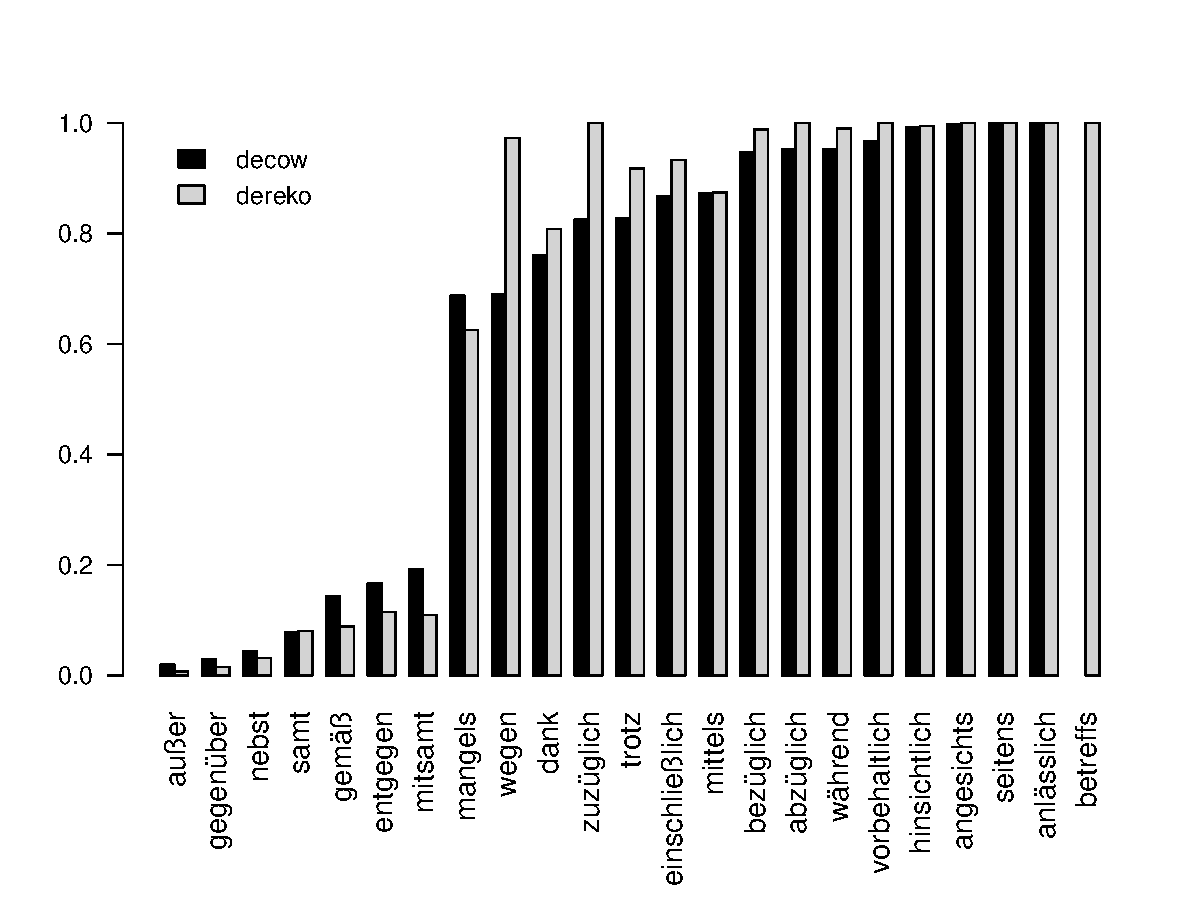
\includegraphics[scale=.7]{../R/prep-genitive-proportions}
   \label{genprops}
  \caption{Proportion of genitive complements (as opposed to dative) by preposition and corpus, in a sample of 80,000 prepositional phrases from DeReKo and DECOW16B}  
\end{figure}


A fair number (but by no means all) of the selected prepositions show some degree of variation in case assignment. For our final dataset, we selected only those prepositions where the proportion of either genitive or dative ocurrences was between 0.1 and 0.9 in at least one of the corpora. In other words, the amount of variation must be such that at least 10\% of all occurrences of that preposition show the minority, non-modal (and arguably, non-standard) case category. Thus, from among the original 23 prepositions, only 10 were included in the final dataset (\textit{entgegen}, \textit{gem\"a\ss}, \textit{mitsamt}, which typically select a dative complement, as well as \textit{dank}, \textit{einschlie{\ss}lich}, \textit{mangels}, \textit{mittels}, \textit{trotz}, \textit{wegen} and \textit{zuz\"uglich}, which typically select genitive). For this dataset, the overall occurence rate of non-standard case assignment is 15.4 \%.

We first specify two logistic regression models that predict the probability of observing the non-modal/non-standard case category, and which do not distinguish between individual prepositions. First, we use the set of COReX variables, represented as $c_1$ \ldots $c_{60}$ in equation~\ref{glm-allpreps-corex}.

\begin{equation}
\label{glm-allpreps-corex}
  P(nonstandard.case=1) = logit^{-1}(\alpha + \beta_1 c_1 + \beta_2 c_2 + \dots + \beta_{60} c_{60})
\end{equation}

Of the resulting coefficient estimates, 32 are different from 0 at p < 0.05. The Nagelkerke Pseudo-R$^2$ score for this model is 0.28.

For comparison, we use the document factor scores from the factor analysis as shown in equation~\ref{glm-allpreps-fa} (where the terms $f_1$ \ldots $f_7$ represent the factor scores of factors 1 through 7). In this model, all coefficient estimates are significant at the 0.05 level, however, the Nagelkerke R$^2$ score for this model drops to 0.24.

\begin{equation}
\label{glm-allpreps-fa}
  P(nonstandard.case=1) = logit^{-1}(\alpha + \beta_1 f_1 + \beta_2 f_2 + \dots + \beta_{7} f_{7})
\end{equation}


Next, we consider separate models for each preposition, using all 60 COReX features as predictors. Figure~\ref{coeffs-corex-individial} illustrates the distribution of estimates for each preposition, for each coefficient with an associated p-value < .05 and absolute value < 5. As is obvious from the plot, coefficient estimates vary greatly, depending on the preposition. 

\begin{figure}
  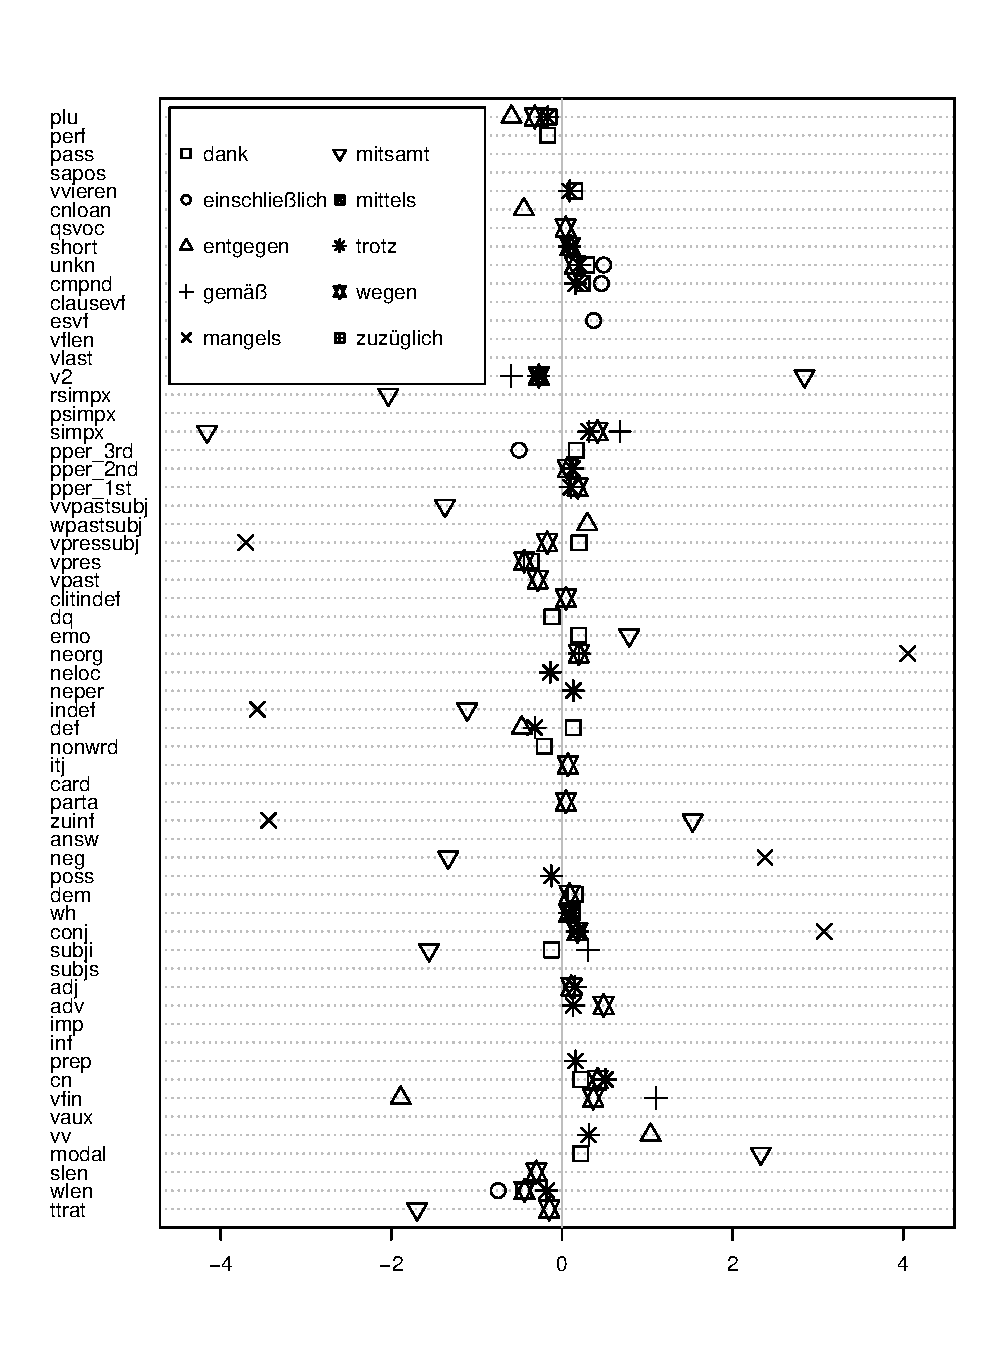
\includegraphics[scale=.9]{../R/prep-individual-coeffs-bw}
  \label{coeffs-corex-individial}
  \caption{COReX features: coefficient estimates with associated p-value $< 0.05$; a separate model was specified for each preposition.}
\end{figure}
\end{document}
